\documentclass{article}
\usepackage[utf8]{inputenc} % Permite el uso de caracteres del Español
\usepackage[T1]{fontenc}
\usepackage{hyperref}
\usepackage{graphicx}
\usepackage{wrapfig}
\usepackage{subcaption}

% Para ecuaciones
\usepackage{amssymb, amsmath, amsbsy} % simbolitos
\usepackage{upgreek} % para poner letras griegas sin cursiva
\usepackage{cancel} % para tachar
\usepackage{mathdots} % para el comando \iddots
\usepackage{mathrsfs} % para formato de letra
\usepackage{stackrel} % para el comando \stackbin

% set font encoding for PDFLaTeX, XeLaTeX, or LuaTeX
\usepackage{ifxetex,ifluatex}
\newif\ifxetexorluatex
\ifxetex
  \xetexorluatextrue
\else
  \ifluatex
    \xetexorluatextrue
  \else
    \xetexorluatexfalse
  \fi
\fi

\ifxetexorluatex
  \usepackage{fontspec}
\else
  \usepackage[T1]{fontenc}
  \usepackage[utf8]{inputenc}
  \usepackage{lmodern}
\fi

% used in maketitle
\title{Actividad 8: Oscilador de Van der Pol}
\author{Melissa Matrecitos Avila}
\date{12 de Abril de 2018}

% Enable SageTeX to run SageMath code right inside this LaTeX file.
% documentation: http://mirrors.ctan.org/macros/latex/contrib/sagetex/sagetexpackage.pdf
% \usepackage{sagetex}

\begin{document}
\maketitle
\section {Introducción - Antecedentes}
El siguiente reporte corresponde a la actividad 8 del curso de Física Computacional 1, en la cual se estudió el oscilador de Van de Pol. Éste sirve para comprender muchos fenómenos naturales interesantes, los cuales poseen soluciones periódicas, o regulares, y se categorizan por ser osciladores. Esto se logro de manera similar a las actividades 6 y 7, resolviendo ecuaciones diferenciales no lineales.

Algunos de los fénomenos mencionados se encuentran, desde hace tiempo, en la física y biología. Uno de ellos fue la aplicación de la ecuación a un campo bidimensional en el modelo de FitzHugh-Nagumo para describir el potencial de acción de las neuronas. También se ha usado en sismología para modelar el comportamiento de dos placas en una falla.

EL reporte presenta una síntesis del artículo completo "Van der Pol oscillator" de  Wikipedia, la exploración de las soluciones del modelo en el espacio fase. También se incluye una pequeña sección con los resultados obtenidos y discusión de estos. Por último se presentan las secciones de conclusión, bibliografía y apéndice.

\section{Modelo de Van der Pol}
El oscilador de Van der Pol es un oscilador con amortiguamiento no lineal. Éste obedece la ecuación diferencial de segundo orden:
\begin{center}
$ {d^{2}x \over dt^{2}}-\mu (1-x^{2}){dx \over dt}+x=0$
\end {center}
en la que x es la posición, función del tiempo t, y $\mu$ es un parámetro escalar para el amortiguamiento. Este modelo fue propuesto por Balthasar Van der Pol (1889-1959) en 1920 cuando era un ingeniero que trabaja para la compañía Philips (en los Países Bajos).

\subsection {Historia}
Cómo se menciono anteriormente, el oscilador de van der Pol fue descrito por el ingeniero y físico Balthasar Van der Pol mientras trabajaba en Philips. El científico encontró oscilaciones estables, que llamó oscilaciones de relajación, las cuales ahora son conocidas como ciclos límite, en circuitos que usaban válvulas de vacío. Cuando esos circuitos se hacen funcionar cerca del ciclo límite entran en acoplamiento y la señal entra en fase con la corriente. Van der Pol y Van der Mark, informaron en el ejemplar de Nature de septiembre de 1927 que en ciertas frecuencias de conducción se escuchaba un ruido irregular, que más tarde se descubrió que era el resultado de un caos determinista.

\subsection{Forma bidimensional}
Según el teorema de Liénard, el sistema tiene un ciclo límite. Su forma bidimensional se puede encontrar de dos formas, aplicando dos transformaciones distintas, una es: $ y=x-x^{3}/3-{\dot {x}}/\mu$, $y=x-x^{3}/3-{\dot {x}}/\mu $, donde el '.' indica derivada, obteniendo las ecuaciones:
\begin{center}
${\dot {x}}=\mu \left(x-{\frac {1}{3}}x^{3}-y\right)$\\
${\dot {y}}={\frac {1}{\mu }}x$
\end{center}
La forma se basa en la transformación $y = \dot x $, llevándonos a encontrar:
\begin{center}
$\dot x = y$\\
$\dot {y}=\mu (1-x^{2})y-x$
\end{center}

\subsection{Resultados del oscilador no forzado}
Dos de las características más interesantes para este tipo de oscilador se dan cuando: $\mu=0$, ya que no interviene el amortiguamiento y la ecuación toma la forma de un oscilador armónico simple, permitiendo siempre la conservación de la energía. La otra situción es cuando $\mu>0$, porque el sistema entra en un ciclo límite, donde cerca del origen, éste es inestable y, lejos del origen, el sistema está amortiguado.

\subsection{Hamiltoniano para el oscilador Van der Pol}
De igual manera se puede escribir un Hamiltoniano independiente del tiempo para el oscilador, esto se logra aumentándolo a un sistema dinámico autónomo, utilizando una ecuación diferencial no lineal de segundo orden como el que se muestra a continuación:
\begin{center}
${\ddot {x}}-\mu (1-x^{2}){\dot {x}}+x=0$\\
${\ddot {y}}+\mu (1-x^{2}){\dot {y}}+y=0$
\end{center}

El oscilador no se ve afectado debido al acoplamiento unidireccional entre las evoluciones temporales de las variables x e y.  Se puede demostrar que una H Hamiltoniana para este sistema de ecuaciones es:
\begin{center}
$H(x,y,p_{x},p_{y})=p_{x}p_{y}+xy-\mu (1-x^{2})yp_{y}$
\end{center}

donde $p_{x} y p_{y}$ son los momentos conjugados correspondientes a x e y, respectivamente. Logrando así una manera de conducir a la cuantificación del oscilador Van der Pol.

\subsection{El oscilador de Van der Pol forzado}
El oscilador de Van der Pol forzado adapta la función 'original' agregando una función de la forma $Asin (\omega t)$, resultando una ecuación diferencial de la forma:
\begin{center}
${d^2x \over dt^2}-\mu(1-x^2){dx \over dt}+x-A \sin(\omega t)= 0$
\end{center}
donde A es la amplitud, o desplazamiento, de la función de onda y $\omega$ es su velocidad angular.
\section{Exploración de las soluciones del modelo en el espacio fase}
Cómo el nombre de la sección indica, se exploró el comportamiento del oscilador, creando gráficas de posición contra tiempo, la fase y ciclo límite de ésta. Para esto se utilizó código muy parecido al de las actividades 6 y 7.

Las primeras dos gráficas del artículo se producieron mediante la creación de archivos que tuvieran datos con distintas condiciones iniciales o bien, distinto coeficiente de amortiguamiento. En especial para la primera gráfica se realizaron distintas imagénes para observar mejor lo que ocurría con el cambio de condiciones iniciales.
La función utilizada en las gráficas del oscilador sin amortiguamiento fue:
\begin{center}
  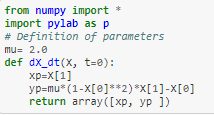
\includegraphics[width=0.4\textwidth]{Funcion.PNG}
\end{center}
Mientras que el código para crear los archivos con datos fue:
\begin{center}
  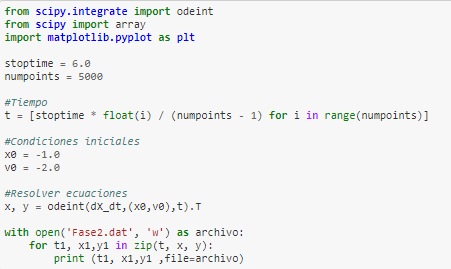
\includegraphics[width=0.8\textwidth]{Archivos.PNG}
\end{center}
En el caso de la primera gráfica, donde se observa el campo de dirección, se utilizó el siguiente código, donde a cada punto se le asigna un vector de dirección:
\begin{center}
  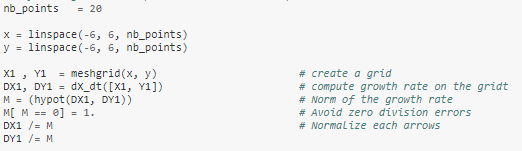
\includegraphics[width=0.7\textwidth]{Malla.PNG}
\end{center}
La siguiente imagen muestra la fase del oscilador de Van der Pol no forzado, junto con un ciclo límite y el campo de dirección:
\begin{center}
  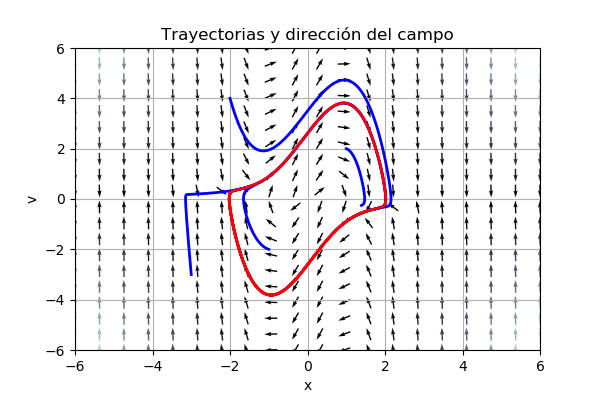
\includegraphics[width=1\textwidth]{FasesCondiciones.png}
\end{center}
Cómo se mencionó anteriormente se crearon algunas gráficas del mismo tipo pero con condiciones iniciales distintas, las cuales fueron:
\begin{center}
  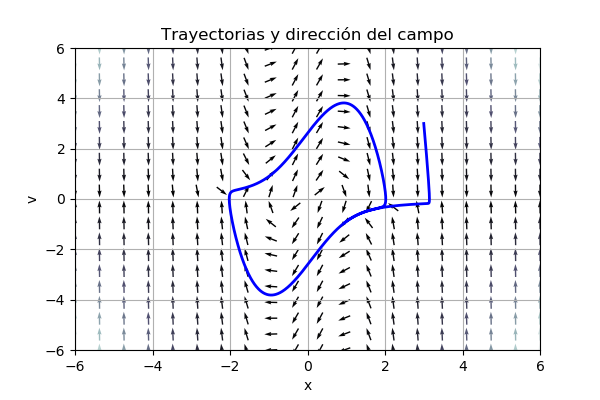
\includegraphics[width=0.45\textwidth]{Prueba1.png}
  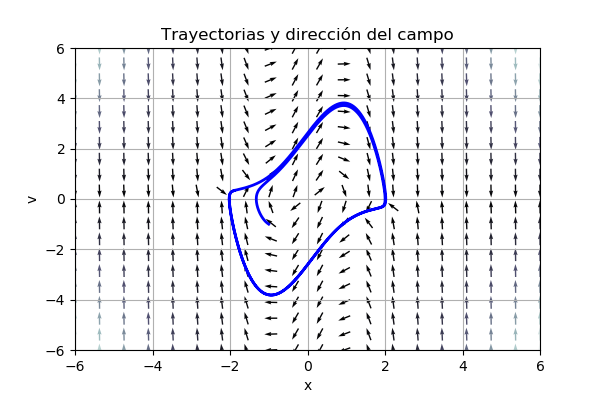
\includegraphics[width=0.45\textwidth]{Prueba2.png}
  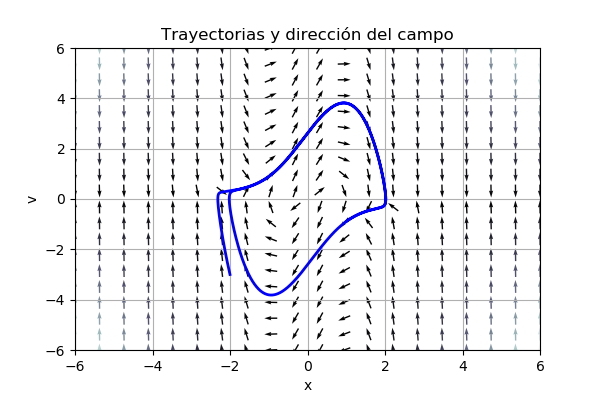
\includegraphics[width=0.45\textwidth]{Prueba3.png}
  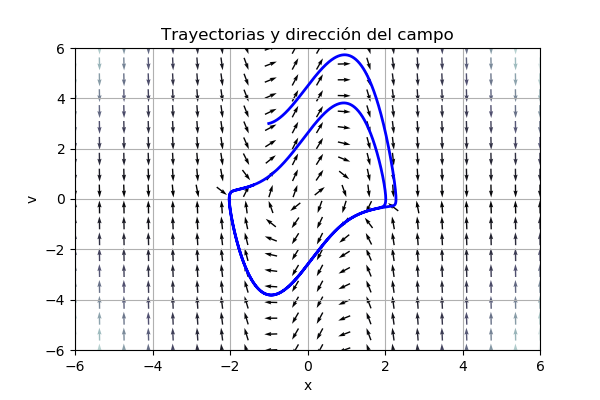
\includegraphics[width=0.45\textwidth]{Prueba4.png}
\end{center}
Para la segunda imagen del artículo, se preocedió igual que para la primera imagen, solo que en lugar de cambiar las condiciones de posición y velocidad, se cambiaron los valores del coeficiente de amortiguamiento, obteniendo:
\begin{center}
  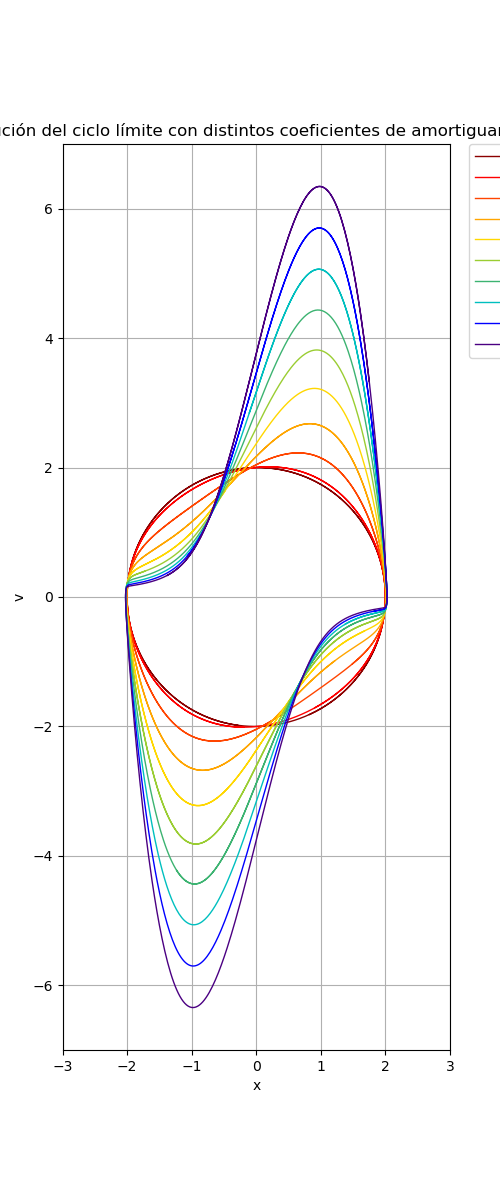
\includegraphics[width=0.75\textwidth]{Coeficientes.png}
\end{center}
En el caso de la tercera imagen, se muestra la oscilación de relajación en el oscilador Van der Pol sin forzamiento externo, con coeficiente de amortiguamiento $\mu=5$:
\begin{center}
  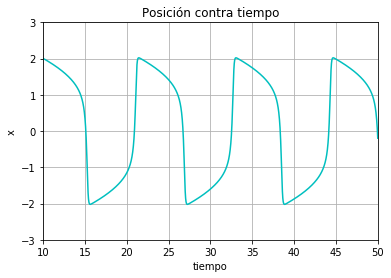
\includegraphics[width=0.75\textwidth]{Posicion_contra_tiempo.png}
\end{center}
Por último, se muestra el comportamiento caótico en el oscilador Van der Pol con forzamiento sinusoidal. El parámetro de amortiguación no lineal es igual a $\mu=8.53$, mientras que el forzamiento tiene una amplitud A = 1.2 y una frecuencia angular $\omega = 2\pi / 10$. Para realizar está gráfica se tuvo que cambiar la función a integrar ya que ahora presenta un término nuevo debido al amortiguamiento:
\begin{center}
  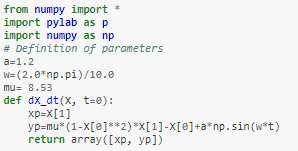
\includegraphics[width=0.6\textwidth]{Funcion2.PNG}
\end{center}
Resultando la gráfica:
\begin{center}
  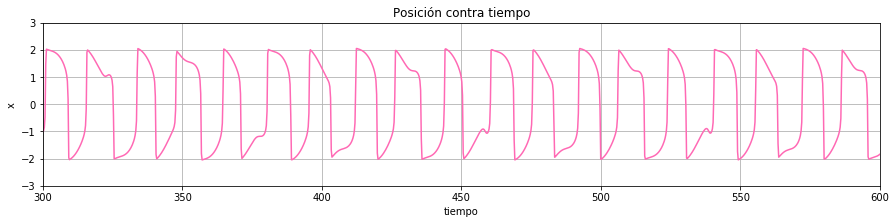
\includegraphics[width=1.2\textwidth]{Posicion_contra_tiempo2.png}
\end{center}
\section{Resultados}
Al realizar la primera imagen del artículo, se puede observar como a pesar de tener distintas condiciones iniciales, el movimiento siempre llega al ciclo límite, solo que unas en menor tiempo que otras. Además el campo direccional nos da indicios de como será la trayectoria de la fase, facilitando la comprensión de la forma del ciclo límite.

La segunda imagen hace notorio el efecto del coeficiente de amortiguamiento en el oscilador, ya que cuando este es pequeño, el ciclo límite es parecido al del oscilador común, pero conforme el coeficiente crece, los picos de la figura se hacen más pronunciados.

Para finalizar, las gráficas 3 y 4, muestran el comportamiento de la posición con respecto al tiempo, donde el oscilador no forzado tiene un comportamiento periódico, mientras que el forzado presenta cambios muy notorios en su trayectoria.

\section{Conclusiones}
El tema me pareció muy interesante ya que era algo nuevo para mi, además de que fue un claro ejemplo de como las condiciones iniciales o un parámetro pueden cambiar la solcución drásticamente. Esto aunado a la la explicación del caos determinista que venía en los artículos, lo hizo aun más atractivo.

De las tres actividades que se realizaron de acuerdo al tema de sistemas de ecuaciones diferenciales no lineales, la actividad 8 fue la que me pareció más complicada, esto debido a que era un código nuevo, sobre todo lo referente a la gráfica del campo direccional. Sin embargo fue más gratificante ver los resulados de la actividad comparada con las dos pasadas.

\section{Bibliografía}
\begin{itemize}
\item Van der Pol oscillator. (2018). En.wikipedia.org. Recuperado el 11 de Abril de 2018, de \url{https://en.wikipedia.org/wiki/Van_der_Pol_oscillator}
\item Matplotlib: lotka volterra tutorial — SciPy Cookbook documentation. (2018). Scipy-cookbook.readthedocs.io. Recuperado el 11 de Abril de 2018, de \url{http://scipy-cookbook.readthedocs.io/items/LoktaVolterraTutorial.html}
\item Van der Pol oscillator. (2018). www.scholarpedia.org Recuperado el 11 de Abril de 2018, de \url{http://www.scholarpedia.org/article/Van_der_Pol_oscillator}
\end{itemize}

\section{Apéndice}
\begin{enumerate}

\item Este ejercicio pareciera similar al desarrollado en las actividades 6 y 7. ¿Qué aprendiste nuevo?

Lo más sobresaliente fue producir la malla correspondiente al campo direccional en la primera imagen, ya que esto no lo había realizado antes.

\item ¿Qué fue lo que más te llamó la atención del oscilador de Van der Pol?

La influencia que tenían las condiciones iniciales y el coeficiente de amortiguamiento en el oscilador, ya que equeños cambios en estas producían gráficas muy distintas, pero al final se llegaba a la misma solución.

\item Has escuchado ya hablar de caos. ¿Por qué sería importante estudiar este oscilador?

Considero que la pirncipal razón para estudiarlo es por las aplicaciones que este puede tener, no sólo en la física si no en otras ramas de la ciencia como la biología.

\item ¿Qué mejorarías en esta actividad?

No le cambiaría nada, por que ya teníamos las bases de las actividades pasadas y se agrego lo de la malla, lo que hizo de esta actividad la más retadora.

\item¿Algún comentario adicional antes de dejar de trabajar en Jupyter con Python?

Trabajar con Python fue muy diferente a como trabajé con Fortran, siento que aún me queda mucho por aprender ya que tiene muchisímas cosas que ofrecer, sin embargo me pareció una gran herramienta que estoy segura seguiré utilizando. Con referencia a trabajar en Jupyter fue un cambio radical con referencia a lo que estaba acostumbrada, obviamente un cambio positivo por que era un entorno muy amigable.

\item Cerramos la parte de trabajo con Python ¿Que te ha parecido?

Me pareció una herramienta muy eficaz y sencilla de comprender, además de que tiene muchas aplicaciones de gran utilidad en la física, que van más allá del análisis de datos.
\end{enumerate}

\end{document}
